\documentclass[11pt,a4paper]{article}

% -- Packages ------------------------------------------------------------------
\usepackage[margin=2.5cm]{geometry}
\usepackage[T1]{fontenc}
\usepackage[utf8]{inputenc}
\usepackage{hyperref}
\usepackage{booktabs}
\usepackage{tabularx}
\usepackage{longtable}
\usepackage{array}
\usepackage{enumitem}
\usepackage{graphicx}
\usepackage{xcolor}
\usepackage{titlesec}
\usepackage{fancyhdr}
\usepackage{mdframed}
\usepackage{tikz}
\usetikzlibrary{positioning}
\usepackage{multirow}
\usepackage{amsmath}
\usepackage{listings}
\usepackage{parskip}

% -- Colors --------------------------------------------------------------------
\definecolor{primary}{RGB}{30, 90, 160}
\definecolor{accent}{RGB}{220, 60, 30}
\definecolor{lightgray}{RGB}{245, 245, 245}
\definecolor{darkgray}{RGB}{80, 80, 80}
\definecolor{green}{RGB}{0, 140, 70}
\definecolor{orange}{RGB}{200, 100, 0}

% -- Section Formatting --------------------------------------------------------
\titleformat{\section}{\Large\bfseries\color{primary}}{}{0em}{}[\color{primary}\titlerule]
\titleformat{\subsection}{\large\bfseries\color{primary}}{}{0em}{}
\titleformat{\subsubsection}{\normalsize\bfseries\color{darkgray}}{}{0em}{}

% -- Header / Footer -----------------------------------------------------------
\pagestyle{fancy}
\fancyhf{}
\rhead{\textcolor{darkgray}{\small Retail AI AR Demos — Setup 1 Design Doc}}
\lhead{\textcolor{darkgray}{\small CONFIDENTIAL DRAFT}}
\cfoot{\thepage}
\renewcommand{\headrulewidth}{0.4pt}

% -- Hyperref Setup ------------------------------------------------------------
\hypersetup{
    colorlinks=true,
    linkcolor=primary,
    urlcolor=primary,
    pdftitle={Retail AI AR Demos – Setup 1 Design Document},
    pdfauthor={Zifeng Wang}
}

% -- Custom Box ----------------------------------------------------------------
\newmdenv[
  backgroundcolor=lightgray,
  linecolor=primary,
  linewidth=1.5pt,
  leftmargin=0, rightmargin=0,
  innerleftmargin=12pt, innerrightmargin=12pt,
  innertopmargin=10pt, innerbottommargin=10pt
]{infobox}

% -- Table Column Types --------------------------------------------------------
\newcolumntype{L}[1]{>{\raggedright\arraybackslash}p{#1}}
\newcolumntype{C}[1]{>{\centering\arraybackslash}p{#1}}

% ══════════════════════════════════════════════════════════════════════════════
\begin{document}
% ══════════════════════════════════════════════════════════════════════════════

% -- Title Page ----------------------------------------------------------------
\begin{titlepage}
  \centering
  \vspace*{2cm}
  {\Huge\bfseries\color{primary} Retail AI AR Demos\\[0.4em]}
  {\LARGE\bfseries Setup 1 — Design Document\\[1em]}
  \textcolor{darkgray}{\large\textit{All Models on Mobile Phone · Open-Source Deployable Stack}}\\[2em]
  \hrule height 1.5pt \vspace{0.5em}
  \begin{tabular}{ll}
    \textbf{Project}   & Retail AI AR Demos                    \\
    \textbf{Scope}     & Setup 1: Stream + On-Device Inference \\
    \textbf{Status}    & DRAFT                                 \\
    \textbf{Devices}   & RayNeo X3 Pro + Android Phone         \\
    \textbf{Author}    & Zifeng Wang                           \\
    \textbf{Date}      & February 2026                         \\
  \end{tabular}
  \vspace{0.5em}\hrule height 1pt
  \vfill
  {\small\textcolor{darkgray}{UltronAI — Internal Use Only}}
\end{titlepage}

\tableofcontents
\newpage

% ══════════════════════════════════════════════════════════════════════════════
\section{Problem Statement}
% ══════════════════════════════════════════════════════════════════════════════

\subsection{Background}

Retail environments face two recurring challenges:

\begin{enumerate}
  \item \textbf{Shoppers} need quick, accurate information about products ---
        nutrition facts, allergens, price --- without scanning barcodes or reading
        small-print labels.
  \item \textbf{Store associates} spend significant time locating misplaced
        products and verifying shelf compliance against planograms, without any
        real-time guidance tool.
\end{enumerate}

Augmented Reality (AR) glasses provide a hands-free, first-person view of the
retail environment. Combined with an AI pipeline, they can surface contextual
information directly in the associate's or shopper's field of view --- or via
voice --- without interrupting the natural workflow.

\subsection{Problem Definition}

\begin{infobox}
\textbf{Core problem:} How to run a complete AI pipeline (video ingestion,
product detection, OCR, retrieval-augmented generation, speech I/O) on
\emph{commodity hardware} (AR glasses + Android phone) with \emph{no dependency
on cloud infrastructure or proprietary APIs}, at latency acceptable for
real-time retail interaction.
\end{infobox}

\subsection{Out of Scope (Setup 1)}

\begin{itemize}[noitemsep]
  \item Running models on the glasses (Setup 2).
  \item Cloud-based LLM or cloud STT/TTS.
  \item Barcode scanning (may be added as Phase 3 enhancement).
  \item Multi-user sessions / back-office analytics dashboard.
\end{itemize}

% ══════════════════════════════════════════════════════════════════════════════
\section{Requirements}
% ══════════════════════════════════════════════════════════════════════════════

\subsection{Functional Requirements}

\subsubsection{FR-1 · Video Streaming}
\begin{itemize}[noitemsep]
  \item The AR glasses shall stream live camera feed to the phone over local
        WiFi (or phone hotspot) using MJPEG over HTTP.
  \item The phone shall display the incoming stream in real time.
\end{itemize}

\subsubsection{FR-2 · Product Detection}
\begin{itemize}[noitemsep]
  \item The phone shall run a real-time object detection model on each incoming
        frame to locate and classify retail products.
  \item Detection results (bounding boxes, class labels, confidence scores)
        shall be overlaid on the live stream view.
\end{itemize}

\subsubsection{FR-3 · OCR on Product Labels}
\begin{itemize}[noitemsep]
  \item Upon user trigger (tap or voice command), the phone shall run OCR on
        the region of interest (detection bounding box crop) to extract text:
        nutrition facts, ingredients, allergen warnings, price.
  \item Raw OCR text shall be passed to the RAG pipeline as additional context.
\end{itemize}

\subsubsection{FR-4 · Speech-to-Text (STT)}
\begin{itemize}[noitemsep]
  \item The phone shall capture voice input from its microphone.
  \item STT shall convert audio to text entirely on-device (no cloud API).
  \item Transcript shall be forwarded to the LLM/RAG pipeline.
\end{itemize}

\subsubsection{FR-5 · Retrieval-Augmented Generation (RAG)}
\begin{itemize}[noitemsep]
  \item The phone shall maintain a local knowledge base of retail products
        (nutrition, allergens, pricing) and shelf planograms.
  \item Given a user query + OCR context, the system shall retrieve the top-$k$
        relevant documents using embedding similarity.
  \item Retrieved context shall be injected into the LLM prompt.
\end{itemize}

\subsubsection{FR-6 · On-Device LLM}
\begin{itemize}[noitemsep]
  \item The phone shall run a quantized open-source LLM locally.
  \item The LLM shall answer user queries using only the retrieved context
        (no hallucination outside provided documents).
  \item Use-case 1 (Shopping Assist): answer questions about nutrition and
        allergens.
  \item Use-case 2 (Shelf Analysis): analyze detected products vs.\ planogram
        and generate associate guidance.
\end{itemize}

\subsubsection{FR-7 · Text-to-Speech (TTS)}
\begin{itemize}[noitemsep]
  \item The phone shall convert LLM output to speech and play it via the phone
        speaker or earphone.
  \item TTS shall run entirely on-device.
\end{itemize}

\subsubsection{FR-8 · Shelf Analysis}
\begin{itemize}[noitemsep]
  \item The system shall detect products on a shelf segment and compare their
        positions to a configurable planogram (zone $\rightarrow$ expected SKU mapping).
  \item Misplaced or missing items shall be identified and reported to the
        associate via voice and on-screen list.
\end{itemize}

\subsection{Non-Functional Requirements}

\begin{table}[h!]
\centering
\renewcommand{\arraystretch}{1.3}
\begin{tabularx}{\textwidth}{L{2.5cm} L{5cm} L{6.5cm}}
\toprule
\textbf{ID} & \textbf{Requirement} & \textbf{Target} \\
\midrule
NFR-1 & End-to-end voice latency & $< 4$\,s from speech end to TTS playback \\
NFR-2 & Detection frame rate    & $\geq 8$\,FPS on mid-range Android (Snapdragon 8 Gen 1+) \\
NFR-3 & Network dependency      & Zero cloud calls; local WiFi only (glasses $\leftrightarrow$ phone) \\
NFR-4 & LLM model size          & $\leq 4$\,GB RAM footprint on phone \\
NFR-5 & Offline operation       & Full pipeline operational with no internet (phone hotspot OK) \\
NFR-6 & Battery                 & $\geq 2$\,h continuous operation on phone \\
NFR-7 & Privacy                 & No user data leaves the local network \\
NFR-8 & Open-source stack       & All models/frameworks must be open-source and self-hostable \\
\bottomrule
\end{tabularx}
\caption{Non-Functional Requirements}
\end{table}

% ══════════════════════════════════════════════════════════════════════════════
\section{High-Level Approach \& Detailed Design}
% ══════════════════════════════════════════════════════════════════════════════

\subsection{System Architecture Overview}

\begin{infobox}
\textbf{Core principle:}
The AR glasses act purely as a \emph{camera + display node}.
The Android phone is the \emph{inference hub} — every AI component runs
on-device. No cloud service is required.
\end{infobox}

\vspace{1em}
\textbf{Data Flow Diagram (Setup 1):}

% Node layout (absolute coordinates, 3-col x 4-row grid, no overlaps):
%
%  Row 0:  [AR Glasses]  -->  [MjpegClient]  -->  [Detector]
%  Row 1:  [STT]         -->  [RAG]          <--  [OCR]
%  Row 2:                     [LLM]
%  Row 3:                     [TTS]
%
\begin{center}
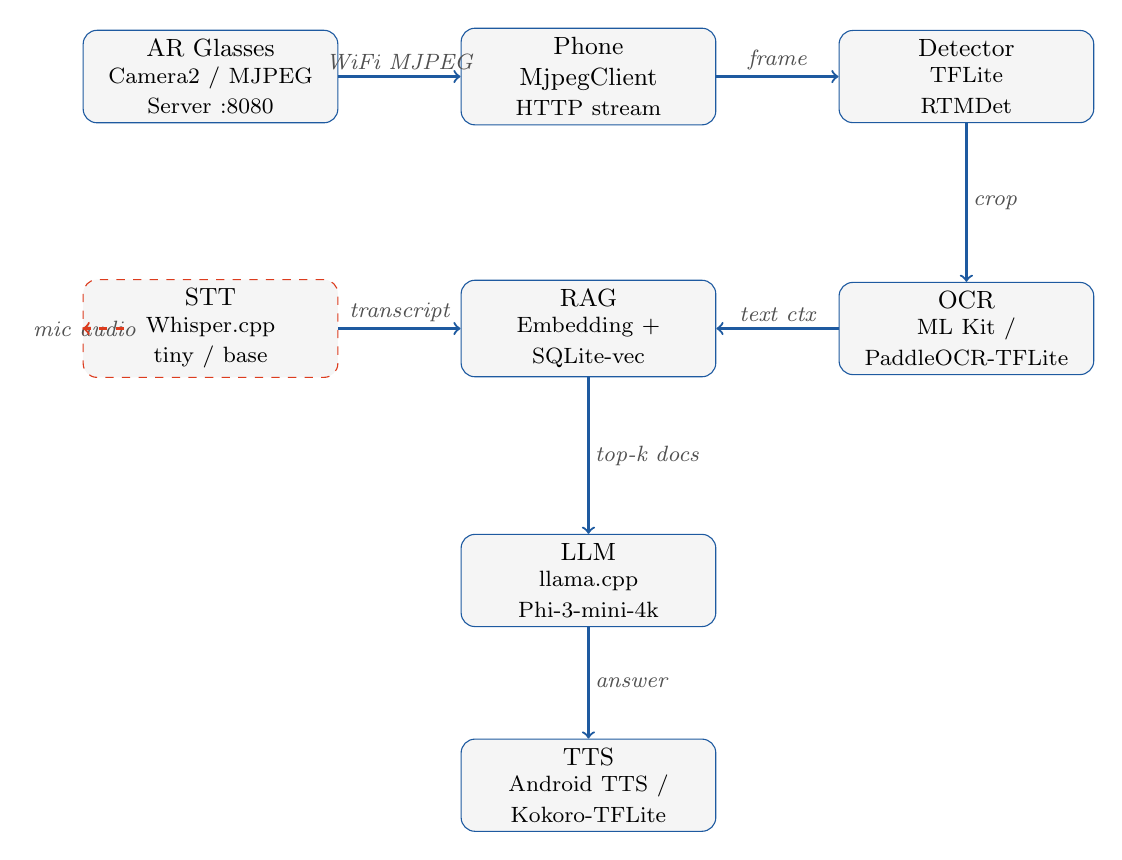
\begin{tikzpicture}[
  box/.style  = {rectangle, rounded corners=5pt, draw=primary, fill=lightgray,
                 text width=3.0cm, align=center, minimum height=1.1cm, font=\small},
  mic/.style  = {rectangle, rounded corners=5pt, draw=accent, fill=lightgray,
                 text width=3.0cm, align=center, minimum height=1.1cm, font=\small,
                 dashed},
  arrow/.style = {->, thick, color=primary},
  lbl/.style   = {font=\footnotesize\itshape, color=darkgray, inner sep=2pt}
]
  % ---- Row 0: video pipeline ----
  \node[box] at (0,   0)    (glasses) {AR Glasses\\{\footnotesize Camera2 / MJPEG\\Server :8080}};
  \node[box] at (4.8, 0)    (stream)  {Phone\\MjpegClient\\{\footnotesize HTTP stream}};
  \node[box] at (9.6, 0)    (detect)  {Detector\\{\footnotesize TFLite\\RTMDet}};

  % ---- Row 1: OCR / RAG / STT ----
  \node[box] at (9.6, -3.2) (ocr)     {OCR\\{\footnotesize ML Kit /\\PaddleOCR-TFLite}};
  \node[box] at (4.8, -3.2) (rag)     {RAG\\{\footnotesize Embedding +\\SQLite-vec}};
  \node[mic] at (0,   -3.2) (stt)     {STT\\{\footnotesize Whisper.cpp\\tiny / base}};

  % ---- Row 2: LLM ----
  \node[box] at (4.8, -6.4) (llm)     {LLM\\{\footnotesize llama.cpp\\Phi-3-mini-4k}};

  % ---- Row 3: TTS ----
  \node[box] at (4.8, -9.0) (tts)     {TTS\\{\footnotesize Android TTS /\\Kokoro-TFLite}};

  % ---- Mic input label (not a node dependency) ----
  \node[lbl] at (-1.6, -3.2) {\textit{mic audio}};

  % ---- Arrows ----
  \draw[arrow] (glasses) -- node[above, lbl]{WiFi MJPEG} (stream);
  \draw[arrow] (stream)  -- node[above, lbl]{frame}      (detect);
  \draw[arrow] (detect)  -- node[right, lbl]{crop}       (ocr);
  \draw[arrow] (ocr)     -- node[above, lbl]{text ctx}   (rag);
  \draw[arrow] (stt)     -- node[above, lbl]{transcript} (rag);
  \draw[arrow] (rag)     -- node[right, lbl]{top-k docs} (llm);
  \draw[arrow] (llm)     -- node[right, lbl]{answer}     (tts);

  % ---- Mic arrow into STT ----
  \draw[arrow, color=accent, dashed] (-1.1,-3.2) -- (stt);
\end{tikzpicture}
\end{center}

\subsection{Component Design}

\subsubsection{Component 1 — Video Streaming}

\begin{table}[h!]
\renewcommand{\arraystretch}{1.3}
\begin{tabularx}{\textwidth}{L{3cm} X}
\toprule
\textbf{Role} & Glasses push live MJPEG to phone over WiFi \\
\textbf{Glasses side} & \texttt{MjpegServer} (existing): Camera2 API $\rightarrow$ JPEG frames $\rightarrow$ HTTP multipart stream on port 8080; dual-Surface for RayNeo left/right eye preview \\
\textbf{Phone side} & \texttt{MjpegClient} (existing): HTTP GET \texttt{/stream}, parse multipart, decode JPEG to \texttt{Bitmap}, deliver to pipeline \\
\textbf{Frame throttle} & Phone-side throttle: process at most 1 frame per 80\,ms ($\approx$12\,FPS) for inference; display at stream rate \\
\textbf{IP discovery} & Glasses display own IP via \texttt{NetworkInterface} fallback; user enters IP once in phone app \\
\bottomrule
\end{tabularx}
\end{table}

\subsubsection{Component 2 — Product Detection}

\begin{table}[h!]
\renewcommand{\arraystretch}{1.3}
\begin{tabularx}{\textwidth}{L{3cm} X}
\toprule
\textbf{Model} & RTMDet-pico (fp16), \texttt{rtmdet\_pico\_fp16.tflite} (existing) \\
\textbf{Framework} & TensorFlow Lite + GPU delegate (fp16) \\
\textbf{Input} & 640×640 px, BGR normalized \\
\textbf{Output} & Rotated bounding boxes (cx, cy, w, h, angle), class id, confidence \\
\textbf{Post-process} & NMS (IoU 0.45, score 0.30); rotated box drawing \\
\textbf{Frame skip} & \texttt{detectWithSkip}: atomic lock, skip frame if previous not done \\
\textbf{Upgrade path} & Swap to retail-trained model (see §4) \\
\bottomrule
\end{tabularx}
\end{table}

\subsubsection{Component 3 — OCR}

\begin{table}[h!]
\renewcommand{\arraystretch}{1.3}
\begin{tabularx}{\textwidth}{L{3cm} X}
\toprule
\textbf{Trigger} & User voice command "analyze this" or single tap \\
\textbf{Input} & Cropped Bitmap from highest-confidence detection box \\
\textbf{Primary option} & \textbf{ML Kit Text Recognition v2} (on-device, no network): Google's on-device OCR; Latin script + digits; returns \texttt{Text} blocks with bounding boxes \\
\textbf{Fallback option} & PaddleOCR TFLite export (see §4 for trade-off) \\
\textbf{Output} & Raw text string passed to RAG pipeline as \texttt{ocrContext} \\
\textbf{Post-process} & Simple keyword filter: extract lines containing allergen keywords (e.g. "nuts", "milk", "gluten") and nutrition facts pattern (\texttt{\textbackslash d+\textbackslash s*(g|mg|kcal)}) \\
\bottomrule
\end{tabularx}
\end{table}

\subsubsection{Component 4 — Speech-to-Text (STT)}

\begin{table}[h!]
\renewcommand{\arraystretch}{1.3}
\begin{tabularx}{\textwidth}{L{3cm} X}
\toprule
\textbf{Model} & \textbf{Whisper.cpp} — \texttt{ggml-tiny.bin} (75\,MB) or \texttt{ggml-base.bin} (142\,MB) \\
\textbf{Integration} & Whisper.cpp Android JNI bindings or pre-built AAR \\
\textbf{Trigger} & "Ask" button or glasses temple single-click $\rightarrow$ start recording; double-click or button again $\rightarrow$ stop \\
\textbf{Audio format} & 16\,kHz, mono, 16-bit PCM; record with \texttt{AudioRecord} \\
\textbf{Latency} & tiny model: $\approx 0.5$\,s for 5\,s audio on Snapdragon 8 Gen 1 \\
\textbf{Language} & English (switchable via \texttt{language} param) \\
\bottomrule
\end{tabularx}
\end{table}

\subsubsection{Component 5 — RAG (Retrieval-Augmented Generation)}

\paragraph{Knowledge Base}

\begin{table}[h!]
\renewcommand{\arraystretch}{1.3}
\begin{tabularx}{\textwidth}{L{3cm} X}
\toprule
\textbf{Data sources} & (1) Product DB: name, SKU, brand, ingredients, nutrition facts, allergen flags; (2) Shelf planogram: zone id $\rightarrow$ expected SKU list, description \\
\textbf{Format} & JSON files bundled in \texttt{app/src/main/assets/}; loaded into SQLite on first run \\
\textbf{Update path} & Replace JSON files and rebuild, or REST pull from store backend (future) \\
\bottomrule
\end{tabularx}
\end{table}

\paragraph{Embedding Model}

\begin{table}[h!]
\renewcommand{\arraystretch}{1.3}
\begin{tabularx}{\textwidth}{L{3cm} X}
\toprule
\textbf{Model} & \textbf{all-MiniLM-L6-v2} converted to TFLite (22\,MB); 384-dim embeddings \\
\textbf{Indexing} & At startup: embed each document chunk $\rightarrow$ store vector in SQLite (\texttt{sqlite-vec} extension) or plain \texttt{BLOB} column \\
\textbf{Query embedding} & At query time: embed (query + OCR text); cosine similarity against stored vectors \\
\textbf{Top-k} & Retrieve top-3 most relevant chunks; concatenate as context \\
\bottomrule
\end{tabularx}
\end{table}

\subsubsection{Component 6 — On-Device LLM}

\begin{table}[h!]
\renewcommand{\arraystretch}{1.3}
\begin{tabularx}{\textwidth}{L{3cm} X}
\toprule
\textbf{Model} & \textbf{Phi-3-mini-4k-instruct} (Q4\_K\_M quantized, $\approx$2.2\,GB); strong instruction-following, fits most flagship phones \\
\textbf{Framework} & \textbf{llama.cpp} Android JNI or \textbf{MLC-LLM} Android AAR \\
\textbf{Prompt template} &
\texttt{<|system|> You are a retail assistant. Answer ONLY from the provided context. If not in context, say "I don't have that information." \textbackslash n<|context|> \{top-k docs\} \textbackslash n<|ocr|> \{ocr text\} \textbackslash n<|user|> \{question\}} \\
\textbf{Context window} & 4096 tokens (Phi-3-mini-4k); sufficient for 3 product docs + OCR \\
\textbf{Max new tokens} & 256 (Shopping assist: short answers; Shelf: short step-by-step) \\
\textbf{Latency} & $\approx$2–3\,s first-token on Snapdragon 8 Gen 2 with Q4 \\
\bottomrule
\end{tabularx}
\end{table}

\subsubsection{Component 7 — Text-to-Speech (TTS)}

\begin{table}[h!]
\renewcommand{\arraystretch}{1.3}
\begin{tabularx}{\textwidth}{L{3cm} X}
\toprule
\textbf{Primary} & Android \texttt{TextToSpeech} API (system TTS engine, e.g. Google TTS pre-installed) — zero extra model, works offline if voice pack downloaded \\
\textbf{Open-source fallback} & \textbf{Kokoro} TFLite or \textbf{Coqui TTS} small model (e.g. \texttt{tts\_models/en/ljspeech/glow-tts}) for fully self-contained TTS if system TTS is unavailable \\
\textbf{Output} & Phone speaker / Bluetooth earphone \\
\bottomrule
\end{tabularx}
\end{table}

\subsection{Demo Flows}

\subsubsection{Demo A — Shopping Assist Agent}

\begin{enumerate}[noitemsep]
  \item User wears glasses, looks at shelf/product.
  \item Phone streams frames from glasses; RTMDet detects product.
  \item User asks by voice: \textit{"Does this contain nuts?"}
  \item STT (Whisper.cpp) transcribes on-device.
  \item User tap / voice trigger $\rightarrow$ OCR on detected product crop $\rightarrow$ extract ingredient/allergen text.
  \item RAG: embed (query + OCR text) $\rightarrow$ retrieve product record from local DB.
  \item LLM (Phi-3-mini): generate concise answer using retrieved context only.
  \item TTS plays: \textit{"Yes, this product contains tree nuts. Also contains milk."}
  \item Answer text displayed on phone screen.
\end{enumerate}

\subsubsection{Demo B — Shelf Analysis}

\begin{enumerate}[noitemsep]
  \item Associate wears glasses, scans shelf section.
  \item RTMDet detects all visible products; positions mapped to shelf zones by Y-coordinate heuristic.
  \item Compliance engine compares detected products per zone vs.\ planogram JSON.
  \item Misplaced / missing items collected into structured list.
  \item LLM generates associate guidance from planogram context + issue list.
  \item TTS plays: \textit{"Move the orange juice from zone 3 to zone 1, top shelf."}
  \item Misplaced items listed on phone screen with zone instructions.
\end{enumerate}

\subsection{Module Map in Codebase}

\begin{verbatim}
ProductARMobile/app/src/main/java/com/ultronai/productarmobile/
+-- ml/
|   +-- RTMDetDetector.kt          (existing — detection)
|   +-- OcrProcessor.kt            (NEW — ML Kit OCR wrapper)
|   \-- EmbeddingModel.kt          (NEW — all-MiniLM TFLite)
+-- llm/
|   \-- LlmClient.kt               (NEW — llama.cpp / MLC-LLM JNI)
+-- rag/
|   +-- KnowledgeBase.kt           (NEW — load product/planogram JSON)
|   +-- VectorStore.kt             (NEW — SQLite-vec retrieval)
|   \-- RagPipeline.kt             (NEW — orchestrate embed+retrieve)
+-- stt/
|   \-- WhisperStt.kt              (NEW — Whisper.cpp JNI)
+-- tts/
|   \-- TtsManager.kt              (NEW — Android TTS / Kokoro)
+-- shopping/
|   \-- ShoppingAssistAgent.kt     (NEW — orchestrate shopping flow)
+-- shelf/
|   +-- ZoneMapper.kt              (NEW — Y-coord $\rightarrow$ zone)
|   +-- ComplianceEngine.kt        (NEW — detected vs planogram)
|   \-- ShelfAnalysisAgent.kt      (NEW — orchestrate shelf flow)
\-- MainActivity.kt                (existing — extend with new UI)
\end{verbatim}

% ══════════════════════════════════════════════════════════════════════════════
\section{Options \& Trade-offs}
% ══════════════════════════════════════════════════════════════════════════════

\subsection{LLM: llama.cpp vs.\ MLC-LLM vs.\ MediaPipe LLM}

\begin{table}[h!]
\centering
\renewcommand{\arraystretch}{1.3}
\begin{tabularx}{\textwidth}{L{2.6cm} L{3.8cm} L{3.8cm} L{3.8cm}}
\toprule
\textbf{Option} & \textbf{Pros} & \textbf{Cons} & \textbf{Verdict} \\
\midrule
\textbf{llama.cpp + JNI}
  & Widest model support (GGUF); battle-tested; large community; easy quantization
  & JNI setup complexity; no native GPU (CPU/NNAPI only unless patched)
  & \textcolor{green}{\textbf{Recommended (Phase 1)}} \\
\midrule
\textbf{MLC-LLM AAR}
  & OpenCL/Vulkan GPU acceleration; higher throughput; official Android AAR
  & Fewer supported models; larger AAR size; less mature for custom models
  & Good for Phase 2 / performance tuning \\
\midrule
\textbf{MediaPipe LLM Inference}
  & Google-maintained; simple API; good GPU usage
  & Limited model selection; not all open models supported
  & Fallback if above fail \\
\midrule
\textbf{OpenAI-compat API}
  & Zero phone RAM; best quality; fast prototyping
  & Requires network; not privacy-safe; cloud cost
  & Dev/debug only; not production \\
\bottomrule
\end{tabularx}
\caption{LLM Option Comparison}
\end{table}

\subsection{LLM Model Selection}

\begin{table}[h!]
\centering
\renewcommand{\arraystretch}{1.3}
\begin{tabularx}{\textwidth}{L{3cm} C{1.5cm} C{1.5cm} L{5.5cm}}
\toprule
\textbf{Model (Q4\_K\_M)} & \textbf{Size} & \textbf{RAM} & \textbf{Notes} \\
\midrule
Phi-3-mini-4k (3.8B) & 2.2\,GB & 2.6\,GB & \textcolor{green}{\textbf{Recommended}} — strong reasoning, fits Snapdragon 8 Gen 1+ \\
Gemma-2-2B-IT        & 1.5\,GB & 1.8\,GB & Good quality; slightly less reasoning \\
Llama-3.2-1B-Instruct & 0.7\,GB & 1.0\,GB & Very fast; lower quality \\
Llama-3.2-3B-Instruct & 1.9\,GB & 2.2\,GB & Balance of speed and quality \\
\bottomrule
\end{tabularx}
\caption{LLM Model Trade-off (all open-source, GGUF format)}
\end{table}

\subsection{OCR: ML Kit vs.\ PaddleOCR-TFLite}

\begin{table}[h!]
\centering
\renewcommand{\arraystretch}{1.3}
\begin{tabularx}{\textwidth}{L{3cm} L{4.5cm} L{4.5cm} C{2cm}}
\toprule
\textbf{Option} & \textbf{Pros} & \textbf{Cons} & \textbf{Verdict} \\
\midrule
\textbf{ML Kit Text Recognition v2}
  & Native Android; no model file needed; good accuracy on printed text; free offline mode
  & Google dependency; less control over model
  & \textcolor{green}{\textbf{Use}} \\
\midrule
\textbf{PaddleOCR TFLite export}
  & Fully self-contained; excellent accuracy; Apache 2.0
  & Larger APK (+50--100\,MB); integration effort
  & Phase 2 upgrade \\
\bottomrule
\end{tabularx}
\caption{OCR Option Comparison}
\end{table}

\subsection{STT: Whisper.cpp vs.\ Android SpeechRecognizer}

\begin{table}[h!]
\centering
\renewcommand{\arraystretch}{1.3}
\begin{tabularx}{\textwidth}{L{3cm} L{4.5cm} L{4.5cm} C{2cm}}
\toprule
\textbf{Option} & \textbf{Pros} & \textbf{Cons} & \textbf{Verdict} \\
\midrule
\textbf{Whisper.cpp (tiny/base)}
  & Fully offline; consistent accuracy; open-source (MIT)
  & JNI setup; 75--142\,MB model file; no streaming
  & \textcolor{green}{\textbf{Use}} \\
\midrule
\textbf{Android SpeechRecognizer}
  & Zero setup; streaming transcription; fast
  & Requires Google services + network; privacy concern
  & Dev/debug only \\
\bottomrule
\end{tabularx}
\caption{STT Option Comparison}
\end{table}

\subsection{Embedding: all-MiniLM-L6-v2 vs.\ nomic-embed-text}

\begin{table}[h!]
\centering
\renewcommand{\arraystretch}{1.3}
\begin{tabularx}{\textwidth}{L{3.5cm} L{3.5cm} L{3.5cm} C{2cm}}
\toprule
\textbf{Model} & \textbf{Pros} & \textbf{Cons} & \textbf{Verdict} \\
\midrule
\textbf{all-MiniLM-L6-v2}
  & 22\,MB; fast; well-supported TFLite export; 384-dim
  & Lower quality than larger models
  & \textcolor{green}{\textbf{Use}} \\
\midrule
\textbf{nomic-embed-text}
  & Higher quality; Apache 2.0
  & Larger; TFLite port less tested
  & Phase 2 \\
\bottomrule
\end{tabularx}
\caption{Embedding Model Comparison}
\end{table}

\subsection{Detection Model: RTMDet vs.\ Retail-Trained YOLO}

\begin{table}[h!]
\centering
\renewcommand{\arraystretch}{1.3}
\begin{tabularx}{\textwidth}{L{3.5cm} L{3.5cm} L{3.5cm} C{2cm}}
\toprule
\textbf{Model} & \textbf{Pros} & \textbf{Cons} & \textbf{Verdict} \\
\midrule
\textbf{RTMDet-pico (existing)}
  & Already integrated; fast; rotated boxes
  & General-purpose; not retail-trained
  & \textcolor{green}{\textbf{Phase 1}} \\
\midrule
\textbf{YOLOv8n / YOLOv11n fine-tuned on retail}
  & Higher mAP on retail products; TFLite export available
  & Need labelled retail dataset; training time
  & Phase 2 target \\
\bottomrule
\end{tabularx}
\caption{Detection Model Comparison}
\end{table}

% ══════════════════════════════════════════════════════════════════════════════
\section{Rollout Plan \& Risk Register}
% ══════════════════════════════════════════════════════════════════════════════

\subsection{Rollout Plan}

\begin{table}[h!]
\centering
\renewcommand{\arraystretch}{1.4}
\begin{tabularx}{\textwidth}{C{1.2cm} L{3.5cm} L{7cm} C{1.5cm}}
\toprule
\textbf{Phase} & \textbf{Name} & \textbf{Deliverables} & \textbf{Effort} \\
\midrule
\textbf{P0} & \textit{Foundation stable}
  & MJPEG stream + RTMDet detection running stably on phone; frame throttle; IP display fix; TempleAction controls
  & 1 week \\
\midrule
\textbf{P1} & \textit{Voice pipeline}
  & STT (Whisper.cpp JNI); Android TTS; "Ask" button in ProductARMobile; end-to-end voice echo test; RECORD\_AUDIO permission
  & 1--2 weeks \\
\midrule
\textbf{P2} & \textit{LLM on-device}
  & llama.cpp JNI integration; Phi-3-mini-4k GGUF loaded; hard-coded context Q\&A test; latency benchmarks
  & 2 weeks \\
\midrule
\textbf{P3} & \textit{OCR + basic Shopping Assist}
  & ML Kit OCR on detection crop; keyword extraction; LLM prompt with OCR context; Shopping Assist flow (voice $\rightarrow$ OCR $\rightarrow$ LLM $\rightarrow$ TTS)
  & 1--2 weeks \\
\midrule
\textbf{P4} & \textit{RAG pipeline}
  & all-MiniLM TFLite embedding; SQLite-vec store; product/nutrition JSON KB; retrieval + LLM context injection; Shopping Assist with real product data
  & 2 weeks \\
\midrule
\textbf{P5} & \textit{Shelf Analysis demo}
  & Planogram JSON; ZoneMapper (Y-heuristic); ComplianceEngine; ShelfAnalysisAgent; TTS guidance; on-screen misplaced list
  & 1--2 weeks \\
\midrule
\textbf{P6} & \textit{Hardening \& demo polish}
  & End-to-end latency tuning; UX improvements (glasses UI hints via stream back-channel); battery test; retail dataset for detection fine-tune
  & 2 weeks \\
\bottomrule
\end{tabularx}
\caption{Rollout Phases}
\end{table}

\subsection{Risk Register}

\begin{longtable}{C{0.4cm} L{3.8cm} C{1.4cm} C{1.4cm} L{5.5cm}}
\toprule
\textbf{\#} & \textbf{Risk} & \textbf{Prob.} & \textbf{Impact} & \textbf{Mitigation} \\
\midrule
\endfirsthead
\toprule
\textbf{\#} & \textbf{Risk} & \textbf{Prob.} & \textbf{Impact} & \textbf{Mitigation} \\
\midrule
\endhead
\bottomrule
\endfoot

R1 & \textbf{LLM OOM on phone} — Phi-3-mini exceeds available RAM on target device
  & \textcolor{orange}{Med}
  & \textcolor{accent}{High}
  & Profile RAM first; fall back to Llama-3.2-1B (0.7\,GB); implement lazy load + unload \\

R2 & \textbf{llama.cpp JNI integration complexity} — Build system issues, ABI mismatch
  & \textcolor{orange}{Med}
  & \textcolor{orange}{Med}
  & Use pre-built AAR from MLC-LLM or community Android builds; fallback to local HTTP server (Ollama) on phone \\

R3 & \textbf{LLM latency too high} — $>$5\,s first-token unacceptable in demo
  & \textcolor{orange}{Med}
  & \textcolor{orange}{Med}
  & Switch to smaller model (1B or 2B); use MLC-LLM for GPU path; stream tokens to TTS \\

R4 & \textbf{OCR accuracy on product labels} — Poor recognition on curved/reflective packaging
  & \textcolor{orange}{Med}
  & \textcolor{orange}{Med}
  & Pre-process crop (contrast, grayscale, resize); try PaddleOCR TFLite; fall back to barcode lookup \\

R5 & \textbf{WiFi instability} — Stream drops, glasses and phone lose connection
  & \textcolor{green}{Low}
  & \textcolor{accent}{High}
  & Auto-reconnect in MjpegClient; increase socket timeout; prefer phone hotspot over shared WiFi \\

R6 & \textbf{Detection model not retail-ready} — RTMDet misses or misclassifies retail products
  & \textcolor{accent}{High}
  & \textcolor{orange}{Med}
  & For P0--P3: use general model + OCR as fallback; P6: fine-tune YOLOv8n on retail dataset (Roboflow) \\

R7 & \textbf{Whisper.cpp JNI build on ARM64} — NDK/CMake config issues
  & \textcolor{orange}{Med}
  & \textcolor{orange}{Med}
  & Use community Android Whisper AAR (whispercpp-android); fallback to Android SpeechRecognizer in dev \\

R8 & \textbf{Battery drain} — Running stream + detector + LLM $>$ 2\,h
  & \textcolor{orange}{Med}
  & \textcolor{orange}{Med}
  & Throttle detection to 8\,FPS; load LLM only on demand; unload after 30\,s idle \\

R9 & \textbf{Planogram data not available} — No real store planogram for Shelf demo
  & \textcolor{orange}{Med}
  & \textcolor{orange}{Med}
  & Build synthetic planogram JSON for demo environment; demo on a manually arranged shelf \\

R10 & \textbf{RayNeo dual-Surface camera not working} — Single Surface causes blank or frozen preview
  & \textcolor{orange}{Med}
  & \textcolor{orange}{Med}
  & Port Mahjong app dual-Surface startup logic (wait \texttt{surfaceList.size==2} before openCamera) \\

\end{longtable}

\subsection{Success Metrics}

\begin{table}[h!]
\centering
\renewcommand{\arraystretch}{1.3}
\begin{tabularx}{\textwidth}{L{4cm} X}
\toprule
\textbf{Metric} & \textbf{Target} \\
\midrule
End-to-end voice latency & $< 4$\,s (speech end $\rightarrow$ TTS start) \\
Shopping Q\&A accuracy   & Correct allergen / nutrition answer for $\geq 80\%$ of test queries \\
Shelf compliance detection & Correctly identify misplaced item in $\geq 3$ of 4 test scenarios \\
Continuous operation     & $\geq 2$\,h without crash or OOM on target phone \\
Stream frame rate        & $\geq 8$\,FPS detection throughput at steady state \\
Zero cloud dependency    & Pipeline fully functional with no internet connection \\
\bottomrule
\end{tabularx}
\caption{Demo Success Metrics}
\end{table}

% ══════════════════════════════════════════════════════════════════════════════
\appendix
\section{Open-Source Model Inventory}

\begin{table}[h!]
\centering
\renewcommand{\arraystretch}{1.3}
\begin{tabularx}{\textwidth}{L{3cm} L{2.5cm} L{2.5cm} L{2cm} X}
\toprule
\textbf{Component} & \textbf{Model} & \textbf{Framework} & \textbf{License} & \textbf{Source} \\
\midrule
Detection & RTMDet-pico & TFLite & Apache 2.0 & OpenMMLab \\
Detection (P6) & YOLOv8n fine-tuned & TFLite & AGPL-3.0 & Ultralytics \\
OCR & ML Kit v2 & Native Android & Proprietary-free use & Google \\
OCR (P2) & PaddleOCR & TFLite & Apache 2.0 & PaddlePaddle \\
Embedding & all-MiniLM-L6-v2 & TFLite & Apache 2.0 & sentence-transformers \\
LLM & Phi-3-mini-4k & GGUF / llama.cpp & MIT & Microsoft \\
LLM alt & Llama-3.2-3B-Instruct & GGUF / llama.cpp & Llama 3.2 License & Meta \\
STT & Whisper tiny/base & Whisper.cpp & MIT & OpenAI \\
TTS & Android TTS & System API & Proprietary-free use & Google \\
TTS (fallback) & Kokoro & TFLite & Apache 2.0 & hexgrad \\
LLM runtime & llama.cpp & JNI & MIT & ggerganov \\
LLM runtime alt & MLC-LLM & AAR & Apache 2.0 & mlc-ai \\
Vector store & sqlite-vec & Extension & Apache 2.0 & asg017 \\
\bottomrule
\end{tabularx}
\caption{Full Open-Source Model \& Library Inventory}
\end{table}

\section{Phone Hardware Targets}

\begin{table}[h!]
\centering
\renewcommand{\arraystretch}{1.3}
\begin{tabularx}{\textwidth}{L{3.5cm} L{3cm} L{2.5cm} X}
\toprule
\textbf{Device tier} & \textbf{Example} & \textbf{Chip} & \textbf{Expected LLM perf.} \\
\midrule
High (primary target) & Samsung S23 / Pixel 8 Pro & Snapdragon 8 Gen 2 / Tensor G3 & Phi-3-mini Q4: $\approx$2--3\,s TTFT \\
Mid & Samsung A54 / Pixel 7a & Exynos 1380 / Tensor G2 & Use Llama-3.2-1B for $<4$\,s TTFT \\
Low & Snapdragon 778G class & SD 778G & Llama-3.2-1B only; detection at 6\,FPS \\
\bottomrule
\end{tabularx}
\caption{Target Android Hardware}
\end{table}

% ══════════════════════════════════════════════════════════════════════════════
\end{document}
